\documentclass[letterpaper]{article} % DO NOT CHANGE THIS
\usepackage[submission]{aaai2027}  % DO NOT CHANGE THIS
% The serif, sans-serif, and monospaced fonts are loaded automatically by
% aaai2027.sty (newtxtext, helvet, courier). DO NOT add \usepackage{times},
% \usepackage{helvet}, \usepackage{courier}, or any other font package.
\usepackage[hyphens]{url}  % DO NOT CHANGE THIS
\usepackage{graphicx} % DO NOT CHANGE THIS
\urlstyle{rm} % DO NOT CHANGE THIS
\def\UrlFont{\rm}  % DO NOT CHANGE THIS
\usepackage{natbib}  % DO NOT CHANGE THIS AND DO NOT ADD ANY OPTIONS TO IT
\usepackage{caption} % DO NOT CHANGE THIS AND DO NOT ADD ANY OPTIONS TO IT
\frenchspacing  % DO NOT CHANGE THIS
%
\usepackage{algorithm}
\usepackage{algorithmic}
\usepackage{comment}
\usepackage{amsmath,amssymb,amsthm}
%
\usepackage{newfloat}
\usepackage{listings}
\DeclareCaptionStyle{ruled}{labelfont=normalfont,labelsep=colon,strut=off} % DO NOT CHANGE THIS
\lstset{%
	basicstyle={\footnotesize\ttfamily},
	numbers=left,numberstyle=\footnotesize,xleftmargin=2em,
	aboveskip=0pt,belowskip=0pt,%
	showstringspaces=false,tabsize=2,breaklines=true}
\floatstyle{ruled}
\newfloat{listing}{tb}{lst}{}
\floatname{listing}{Listing}
%
\usepackage{booktabs}
%
\pdfinfo{
/TemplateVersion (2027.1)
}

% Theorem environments and notation.
\newtheorem{assumption}{Assumption}
\newtheorem{definition}{Definition}
\newtheorem{proposition}{Proposition}
\newtheorem{corollary}{Corollary}
\newtheorem{lemma}{Lemma}
\newtheorem{theorem}{Theorem}
\newtheorem{example}{Example}
\newtheorem{remark}{Remark}

\newcommand{\Acal}{\mathcal{A}}
\newcommand{\Ecal}{\mathcal{E}}
\newcommand{\ind}{\mathbf{1}}
\newcommand{\R}{\mathbb{R}}
\newcommand{\E}{\mathbb{E}}
\newcommand{\Var}{\operatorname{Var}}

\setcounter{secnumdepth}{0} %May be changed to 1 or 2 if section numbers are desired.

% Title
\title{PFM: Serving Current Personal Facts Under On-Device Latency Budgets}
\author{
    Written by AAAI Press Staff\textsuperscript{\rm 1}\thanks{With help from the AAAI Publications Committee.}\\
    AAAI Style Contributions by Peter Patel Schneider,
    Sunil Issar,\\
    J. Scott Penberthy,
    George Ferguson,
    Hans Guesgen,
    Francisco Cruz\equalcontrib\corresponding,
    Marc Pujol-Gonzalez\equalcontrib\corresponding
}
\affiliations{
    \textsuperscript{\rm 1}Association for the Advancement of Artificial Intelligence\\
    1101 Pennsylvania Ave, NW Suite 300\\
    Washington, DC 20004 USA\\
    proceedings-questions@aaai.org
}

\begin{document}
\maketitle

\begin{abstract}
Persistent memory for on-device language assistants must retrieve facts that are relevant to the current request, correctly attributed, still valid, and available before generation begins. We formulate \emph{deadline-constrained personal fact retrieval}, in which a memory layer selects facts from an evolving personal store subject to prompt and serving-time budgets, and distinguish misattribution, staleness, and lateness as separate failures. We propose Personal Fact Memory (PFM), which stores prompt-ready atomic facts with entity, participant, and temporal metadata, closes superseded values through keyed supersession, retrieves using field-weighted lexical search and bounded local association, and moves model-dependent processing off the serving path. In replay through a deployed macOS autocomplete assistant, PFM places the target fact in the prompt in 24 of 25 scenarios and resolves 8 of 8 identity probes, against 5 of 8 without participant attribution. On a 240-query controlled update benchmark, keyed supersession recalls the current value on every query with zero stale exposure, where a keyless store exposes superseded values on 66\% of queries; under identical corpus, device, and budgets, a local dense retriever exposes stale values on 78\% of requests and cannot meet deadlines below its 15~ms query encoding, while PFM serves its full clean rate from 0.5~ms. Replaying the same prompts through a frozen 7B model, correct completions rise from 0\% without memory to 92.5\% with PFM, with no stale or wrong-person generations, against 35.8\% stale for plain BM25.
\end{abstract}

% Keywords (OpenReview form field only; AAAI main track prints none):
% Personalized Memory Systems; On-Device LLM Agents; Low-Latency
% Retrieval-Augmented Generation; Bi-Temporal Knowledge Representation;
% Real-Time Text Completion
\section{Introduction}

An on-device autocomplete assistant can generate fluent text without knowing the user's facts. Suppose a user replying to Alex types ``The concert is at.'' A useful continuation requires the time Alex and the user most recently agreed on, not a plausible time produced from the model's parametric knowledge. A memory layer can supply that information only if it identifies the correct person, accounts for later revisions, and returns the fact before generation begins. Figure~\ref{fig:teaser} illustrates this setting in the autocomplete assistant studied in this paper.

\begin{figure}[t]
\centering
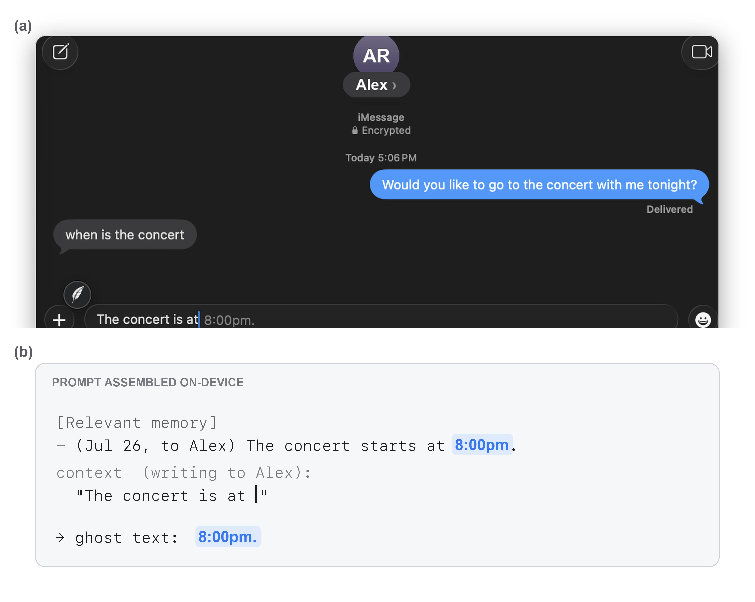
\includegraphics[width=\columnwidth]{figures/teaser.pdf}
\caption{PFM in the deployed autocomplete assistant, with the recipient pseudonymized. The user replies to a question about a concert and types ``The concert is at.'' PFM supplies the remembered time in a compact \texttt{[Relevant memory]} block that is available to the frozen language model when it generates the completion.}
\label{fig:teaser}
\end{figure}

Recent agent-memory systems organize prior interactions through extracted records, temporal graphs, external memory tiers, and associative retrieval \citep{chhikara2025mem0,rasmussen2025zep,gutierrez2024hipporag,packer2023memgpt}. Long-horizon benchmarks such as LongMemEval evaluate whether an assistant can recover information from earlier conversations \citep{wu2024longmemeval}. Real-time personal assistance adds constraints that retrieval accuracy alone does not capture. Similar text may refer to different people, a previously correct fact may become obsolete after an update, and a useful retrieval may arrive after the host model has already started generation. These failures are especially relevant on personal devices, where memory retrieval competes with the language model for limited compute and must operate within an interactive latency budget.

We study this setting as \emph{deadline-constrained personal fact retrieval}. A request contains the local typing context, interaction participants, a personal fact store, a prompt budget, and a serving deadline. The memory layer selects a small set of facts for injection into the prompt. We distinguish misattribution, in which a retrieved fact belongs to the wrong person or entity; staleness, in which an obsolete value is surfaced as current; and lateness, in which otherwise useful context is unavailable by the serving deadline. These errors require evaluation beyond semantic relevance alone.

We propose \textbf{Personal Fact Memory (PFM)} for this setting. PFM stores prompt-ready atomic facts with explicit entity and participant fields and temporal version information. Field-weighted lexical retrieval uses the identities present in the current interaction, and a local entity graph provides an additional association signal when the typed context omits the target entity. Fact extraction and index maintenance run asynchronously, while serving uses only in-memory retrieval and immutable snapshots. No embedding model or language model is invoked on the serving path. When two observations are assigned the same mutable slot key, temporal versioning removes the superseded value from the active index while retaining its history.

We evaluate the memory layer first in isolation and then through the model that consumes its output. In offline replay through the deployed autocomplete data path, PFM places the ground-truth fact in the prompt in 24 of 25 scenarios, and participant-aware retrieval resolves 8 of 8 targeted identity probes against 5 of 8 without the participant field. On a controlled 240-query update benchmark spanning revision depth, paraphrase, cancellation, and identity ambiguity, keyed supersession recalls the current value on every query with zero stale exposure, where the keyless configuration exposes a superseded value on 66.2\% of queries. Under identical corpus, device, and budget conditions, validity-aware lexical serving is the only family that delivers clean facts within millisecond deadlines: a local MiniLM retriever attains the highest current-value recall of any baseline yet exposes stale values on 77.9\% of requests and misses every deadline below its 15~ms query encoding. Replaying the same prompts through a frozen 7B model shows the differences propagate to text: correct completions rise from 0\% without memory to 92.5\% with PFM, with no stale or wrong-person generations, while plain BM25 yields 35.8\% stale completions. These measurements still do not establish that users accept the resulting completions in live use.

We make three contributions.
\begin{enumerate}
\item \textbf{Problem formulation.} We formulate deadline-constrained personal fact retrieval and define misattribution, staleness, and lateness as distinct retrieval failures under prompt and serving-time budgets.
\item \textbf{Memory architecture.} We develop PFM, which combines participant-aware fact representation, temporal versioning for keyed updates, asynchronous memory construction, and a model-free serving path based on in-memory retrieval and immutable snapshots. We state the conditions under which keyed updates maintain a unique active value and the serving protocol bounds memory-induced delay.
\item \textbf{System evidence.} We evaluate PFM through offline replay and mechanism probes in a deployed autocomplete assistant; a controlled update benchmark that measures current-fact recall, stale exposure, and co-injection under keyed revision, paraphrase, and cancellation; baseline comparisons against BM25 variants, a local dense retriever, and a hybrid under identical corpus, device, and deadline budgets, summarized as clean-retrieval rate versus serving deadline; and completion-level replay through a frozen local model that measures correct, stale, and wrong-person generations and time to first token.
\end{enumerate}

\section{Related Work}

\paragraph{Personal and evolving memory.} Long-term agent memory has been built from external stores, structured records, and graph retrieval: MemGPT pages between memory tiers \citep{packer2023memgpt}, Mem0 extracts and updates persistent facts \citep{chhikara2025mem0}, A-MEM stores linked atomic notes \citep{xu2025amem}, and HippoRAG retrieves over an entity graph \citep{gutierrez2024hipporag}; EMG-RAG builds an editable memory graph from smartphone data for a phone assistant \citep{wang2024emgrag}. Temporal consistency is now a direct object of study---Zep maintains a temporal knowledge graph \citep{rasmussen2025zep}, APEX-MEM resolves conflicts in an append-only property graph \citep{banerjee2026apexmem}, Temporal Semantic Memory models event time and durative states \citep{su2026tsm}, and Memora tests reliance on obsolete information after updates \citep{uddin2026memora}. PFM therefore treats neither personalization, graph structure, nor temporal memory as standalone novelty; its focus is the retrieval regime of an interactive assistant, where identity attribution, current validity, and availability before generation must hold on the same request.

\paragraph{Efficient memory serving.} Recent systems treat memory-operation cost as part of the design. Lightweight LLM Agent Memory separates online retrieval from offline consolidation under a fixed retrieval budget \citep{zhang2026lightmem}; AME co-designs vector-memory querying, insertion, and maintenance for mobile hardware \citep{zhao2025ame}; AgentIR adaptively decides when a dense channel is worth its cost \citep{yuan2026agentir}; and system-level profiling shows construction, retrieval, and freshness shifting cost across phases of agent execution \citep{omri2026agentmemory,zhou2026ready}. Making latency explicit narrows the claim for PFM: PFM studies a serving path that uses participant metadata and active temporal state, invokes no embedding or language model at completion time, and falls back to a published snapshot when a fresh retrieval exceeds its waiting budget.

\paragraph{Evaluation of long-term memory.} LoCoMo and LongMemEval test recovery and reasoning over extended histories \citep{maharana2024evaluating,wu2024longmemeval}, and recent work adds temporal validity, obsolete-memory penalties, retrieval efficiency, and phase-level systems cost \citep{uddin2026memora,su2026tsm,huang2026licomemory,omri2026agentmemory}. The autocomplete setting adds application-specific structure: the current participant disambiguates otherwise similar facts, prompt space is limited, and memory must arrive before the completion request proceeds. We therefore evaluate identity errors, stale co-injection, fact availability, and retrieval latency separately rather than as one accuracy measure.

\section{Problem Formulation}

We consider a single user whose personal memory evolves as documents, messages, and other observations arrive over time. At time $t$, let $\mathcal{M}_t$ denote the facts retained by the memory layer, including active facts and facts preserved only as history. A completion request consists of typing context $c_t$, a participant set $P_t$, a serving deadline $\Delta_t$, a maximum number of injected facts $k$, and a character budget $B$. The deadline is the latest time at which retrieved context can be incorporated before the host model begins generation.

\begin{definition}[Personal fact]
A stored fact is a tuple
\begin{equation}
f=(z_f,E_f,P_f,\kappa_f,a_f,b_f,\ell_f),
\end{equation}
where $z_f$ is the prompt-ready text, $E_f$ is a set of normalized entities, $P_f$ is the participant set associated with the source, $\kappa_f$ is an optional key for a mutable semantic slot, $[a_f,b_f)$ is the interval during which the system treats the fact as active, and $\ell_f$ is its prompt length. We set $b_f=\infty$ when a fact has not been superseded. The active view at time $t$ is $\mathcal{A}_t=\{f\in\mathcal{M}_t:a_f\le t<b_f\}$.
\end{definition}

The active interval records the state of the memory system; it does not assert that the stored proposition is true in the world. An extractor may fail to recognize that a new observation revises an earlier one. Semantic validity must therefore be evaluated separately from the system's active view.

A retrieval policy $\pi$ maps $(\mathcal{A}_t,c_t,P_t)$ to an ordered set $S_{\pi,t}\subseteq\mathcal{A}_t$ and incurs serving latency $L_{\pi,t}$. The returned set must satisfy
\begin{equation}
|S_{\pi,t}|\le k, \qquad \sum_{f\in S_{\pi,t}}\ell_f\le B,
\end{equation}
and must be available by $\Delta_t$ to affect the current completion. The prompt constraints limit the amount of memory supplied to the language model, while the deadline limits the time available to obtain it.

For evaluation, let $R_t(f)=1$ when fact $f$ is relevant to request $t$, $I_t(f)=1$ when its entity and participant attribution matches the intended identity of the request, and $V_t(f)=1$ when the proposition remains semantically valid at time $t$. These labels describe ground truth and need not be observable by the retrieval policy. Define
\begin{equation}
\mathcal{G}_t=\{f\in\mathcal{M}_t:R_t(f)=1,\ I_t(f)=1,\ V_t(f)=1\}
\end{equation}
as the set of facts that are relevant, correctly attributed, and valid for request $t$.

\begin{definition}[Deadline-constrained personal fact retrieval]
Retrieval succeeds on request $t$ when at least one fact in $\mathcal{G}_t$ is returned within the serving deadline while satisfying the prompt constraints. Define correct-by-deadline availability as
\begin{equation}
Y^{\mathrm{db}}_{\pi,t}=\mathbf{1}\{S_{\pi,t}\cap\mathcal{G}_t\neq\varnothing\}\mathbf{1}\{L_{\pi,t}\le\Delta_t\}.
\end{equation}
\end{definition}

Misattribution occurs when a retrieved fact is relevant in content but belongs to the wrong identity, $E^{\mathrm{id}}_{\pi,t}=\mathbf{1}\{\exists f\in S_{\pi,t}:R_t(f)=1,\ I_t(f)=0\}$. Staleness occurs when a retrieved fact concerns the intended identity but is no longer valid, $E^{\mathrm{stale}}_{\pi,t}=\mathbf{1}\{\exists f\in S_{\pi,t}:R_t(f)=1,\ I_t(f)=1,\ V_t(f)=0\}$. Lateness occurs when retrieval misses the serving deadline, $E^{\mathrm{late}}_{\pi,t}=\mathbf{1}\{L_{\pi,t}>\Delta_t\}$. The three indicators need not be mutually exclusive. A prompt may contain both a current value and a superseded value, so successful fact retrieval does not by itself imply temporal correctness.

For evaluations with complete identity and validity labels, we also define clean correct-by-deadline retrieval,
\begin{equation}
Y^{\mathrm{clean}}_{\pi,t}=Y^{\mathrm{db}}_{\pi,t}\mathbf{1}\{E^{\mathrm{id}}_{\pi,t}=0\}\mathbf{1}\{E^{\mathrm{stale}}_{\pi,t}=0\}.
\label{eq:clean_deadline}
\end{equation}
This stricter outcome requires the target fact to be available by the deadline without exposing a relevant wrong-identity or stale fact on the same request.

\paragraph{Keyed temporal updates.} Consider a mutable semantic slot with key $\kappa$. Suppose every recognized revision to that slot receives the same key and updates are processed serially. When a new fact $f'$ with key $\kappa$ is inserted at time $s$, the update rule sets $a_{f'}=s$ and $b_{f'}=\infty$. If an active predecessor $f$ with the same key exists, the rule also sets $b_f=s$. The predecessor remains in $\mathcal{M}_t$ as history but is removed from the active view.

\begin{proposition}[Unique active value under keyed supersession]
\label{prop:unique_active_value}
Fix a key $\kappa$. If updates with key $\kappa$ are processed serially by the rule above and the store initially contains at most one active fact with that key, then for every time $t$,
\begin{equation}
\left|\{f\in\mathcal{A}_t:\kappa_f=\kappa\}\right|\le 1.
\end{equation}
\end{proposition}

The claim follows by induction over keyed updates because a new value becomes active at the same instant that the unique active predecessor, if any, is closed. The full proof is given in the supplementary material. The result depends on correct key assignment; it does not guarantee that the extractor identifies every revision or that the newest observation is semantically correct.

\section{Personal Fact Memory}

PFM separates memory construction from memory serving. Construction begins after the system observes a document and may include fact extraction, deduplication, temporal updates, graph maintenance, and pruning. These operations run asynchronously. Serving operates on the resulting in-memory state and does not call an embedding model or language model.

\subsection{Memory Construction}

Each extracted fact carries prompt text, normalized entities, source participants, and an optional key for a mutable semantic slot, as defined in the previous section. In the deployed assistant, the participant field is obtained from the interaction context in which the source document is observed. For supported messaging and mail applications, the active window identifies the interlocutor independently of the words in the document. This metadata is stored with the fact and later used during retrieval.

When a newly extracted fact receives the same slot key as an active fact, PFM applies keyed supersession and removes the predecessor from the active view. Supersession is checked before near-duplicate admission control: a revision that reuses the sentence surface with only the value changed must update the slot, not be absorbed as a re-observation of the old fact. Only an exactly repeated sentence reinforces the current value. Facts for which no reliable slot key is available remain separate observations. Proposition~\ref{prop:unique_active_value} therefore applies to recognized revisions, not to arbitrary pairs of contradictory text.

PFM maintains a fielded inverted index over active facts, with separate fields for prompt text, entities, and participants. It also maintains an entity co-occurrence graph whose edges summarize associations observed in the user's fact store. Index and graph updates occur on the construction path. Historical facts may be retained for provenance, but inactive facts do not enter retrieval.

The implementation also records a fact class and a usage score. Facts are labeled episodic, semantic, or profile for retention purposes. Profile facts are pinned, while other facts may be pruned as recency and use decline. The usage score increases when a completion that used the fact is accepted and decays over time. These quantities are used as ranking and retention signals; the paper does not treat them as evidence for a cognitive model of human memory.

\subsection{Retrieval and Ranking}

For a completion request, PFM constructs a focal query from the tokens preceding the cursor and from the current participant set. Token weights decay with distance from the cursor as $\lambda^d$, with $\lambda=0.95$ in the deployed configuration. Participant terms receive an additional weight of $1.5$, and the query retains at most 12 terms ranked by weighted inverse document frequency. Limiting the query size bounds the amount of query-side work before index traversal.

The lexical retriever uses BM25F \citep{robertson2004simple,robertson2009probabilistic} over the text, entity, and participant fields. The deployed field weights are $1.0$, $2.5$, and $2.0$, respectively. Participant weighting distinguishes facts whose text is similar but whose source interactions involve different people. For example, two messages that both say ``deadline moved to Friday'' can be separated when one was sent to Alice and the other to Bob.

Lexical retrieval is supplemented by bounded one-hop propagation over the entity graph. Let $Q_t$ be the seed entities recovered from the query and participant metadata, and let $w_{eg}(t)$ be the current weight between entities $e$ and $g$. For fact $f$ with entity set $E_f$, PFM computes
\begin{equation}
s_{\mathrm{assoc}}(f\mid Q_t)=\sum_{e\in Q_t}\sum_{g\in E_f}w_{eg}(t),
\end{equation}
with fixed limits on the number of seeds and neighbors traversed. The graph score provides an association signal when the current text names an entity connected to the target fact but does not name the target directly. This differs from full graph ranking methods such as HippoRAG \citep{gutierrez2024hipporag}, which perform broader propagation for open-domain retrieval.

The deployed ranker combines lexical relevance, recency, prior use, and graph association. Let $\Delta t_f$ denote the age of fact $f$, let $h_f(t)$ denote its decaying usage score, and let $T_{\mathrm{rec}}$ be the recency half-life. The score is
\begin{equation}
\mathrm{score}(f)=\mathrm{BM25F}(q_t,f)\left(\varepsilon+(1-\varepsilon)2^{-\Delta t_f/T_{\mathrm{rec}}}\right)\left(1+\eta h_f(t)\right)+\gamma s_{\mathrm{assoc}}(f\mid Q_t),
\label{eq:pfm_score}
\end{equation}
where $\varepsilon$, $\eta$, and $\gamma$ are fixed parameters. The recency floor $\varepsilon$ allows an old fact to remain retrievable when its lexical evidence is strong. The usage term gives more weight to facts that have previously contributed to accepted completions. The experiments ablate these components separately rather than assuming that each improves retrieval.

PFM ranks candidate facts by \eqref{eq:pfm_score} and inserts them in score order until either $k$ facts or $B$ characters have been selected; this greedy rule is the deployed policy. A budget-aware alternative that reallocates prompt space across facts of unequal length, together with its analysis, is presented in the supplementary material.

\subsection{Serving Protocol}

PFM supports snapshot serving and fresh retrieval with bounded waiting. In snapshot mode, a background thread retrieves candidate facts during typing pauses and publishes an immutable result by atomic pointer replacement. When a completion request arrives, the serving thread reads the latest published snapshot and proceeds without waiting for a new retrieval. In fresh mode, the request starts a new retrieval and waits for at most $\delta_t$ before falling back to the latest snapshot. The waiting budget $\delta_t$ is chosen below the request deadline $\Delta_t$.

Let $r$ be an upper bound on the time required to read a published snapshot after the serving thread is scheduled. Assume that published snapshots are immutable, publication uses an atomic pointer replacement, and the serving path acquires no lock held by memory construction or background retrieval.

\begin{proposition}[Bound on memory-induced waiting]
\label{prop:waiting_bound}
Under the assumptions above, snapshot mode adds at most $r$ time to the completion path. Fresh mode adds at most $\delta_t+r$. These bounds do not depend on the duration of fact extraction, index maintenance, graph updates, or pruning.
\end{proposition}

The bound follows because snapshot mode performs only the bounded snapshot read, while fresh mode waits for at most $\delta_t$ before using a fresh result or the latest snapshot. The full proof is given in the supplementary material. Proposition~\ref{prop:waiting_bound} bounds delay introduced by memory serving; it does not guarantee that a fresh result is available by the deadline or that the retrieved facts are correct.

\paragraph{Pruning.} Periodic pruning removes nonprofile facts whose recency and usage scores fall below a configured threshold and deletes the corresponding graph state. This policy reduces inactive or rarely used state in practice, but a threshold rule alone does not impose a deterministic upper bound on memory size under arbitrary arrival patterns. Storage footprint is therefore measured empirically rather than claimed as a consequence of the pruning rule.

\section{Deployment Setting}

PFM is integrated into a commercially deployed macOS autocomplete assistant that offers inline completions in text fields across applications: a greyed continuation appears at the cursor, the user accepts the full completion or a single word, and continued typing dismisses it. This makes the serving constraint concrete---memory must be incorporated before the prompt is handed to the host model---and makes acceptance an observable usage signal. For supported messaging and mail applications the frontmost window title identifies the interlocutor, which PFM records as participant metadata when a sent message is observed and reads again when a later completion is issued; this instantiates the participant set $P_t$ from the interaction context rather than from the words being typed, letting two lexically similar facts be separated when they arose in conversations with different people.

The assistant captures sent text after a send-confirmation event and on application or window transitions, and passes observations asynchronously to memory construction, so extraction, indexing, temporal updates, and pruning never delay the triggering request. Capture excludes password and secure-entry fields, suppresses credential-management applications, and drops secret-like content (API keys, access tokens); the fact store stays on the device. At completion time, PFM serializes the selected facts into a compact \texttt{[Relevant memory]} block in the user-context portion of the prompt, capped at $B$ characters so memory cannot crowd out live context; in snapshot mode the published block is stable across a typing burst, which avoids changing the prompt prefix at every keystroke and can preserve host prompt caching. Acceptance is recorded only when the user adopts a completion and drives the retention and ranking mechanisms above; we treat it as a usage signal, not as evidence that a particular retrieved fact caused the acceptance.

\section{Evaluation}

We evaluate PFM at the memory layer using replay through the deployed assistant's capture and serving paths, and then extend the evaluation along three axes that replay alone cannot support: temporal correctness on a controlled update benchmark, comparison against standard retrieval families under identical corpus, device, and deadline budgets, and completion-level effects through a frozen local language model. Systems-scaling measurements and a budget-aware selection study appear in the supplementary material. The primary replay metric is target fact availability, defined as the fraction of requests for which the prompt contains the ground-truth tokens. This metric is weaker than the clean correct-by-deadline outcome in Eq.~\eqref{eq:clean_deadline} because the replay corpus does not provide exhaustive identity and validity labels for every retrieved candidate. We therefore report targeted identity and stale co-injection probes separately rather than constructing an unsupported clean aggregate.

\subsection{Replay Setup}

A scripted 28-day sequence of sent messages is ingested through the deployed capture path, including the same participant metadata used by the application. The small harness contains 9 captured messages producing 8 indexed facts and 7 completion scenarios. The large harness begins with 31 hand-written seed facts, adds 16 chit-chat messages and 240 synthetic filler messages (287 captured messages in total), and produces 270 indexed facts. The 25 large-harness scenarios span direct recall (20), associative recall where the prefix omits the target entity (2), a conflicting update (1), a CJK entity (1), and one deliberate extraction failure (a sentence lacking a signal verb). Retrieval uses $k=6$ and an 800-character prompt budget.

\subsection{Target Fact Availability}

With memory enabled, the target tokens reach the prompt in 6 of 7 small-harness scenarios and 24 of 25 (96\%) large-harness scenarios; with memory disabled, none of the target facts are present because the live typing context does not contain them (0/7 and 0/25). On the large harness, availability is 20/20 for direct recall, 2/2 associative, 1/1 conflicting-update, and 1/1 CJK; the designed extraction failure accounts for the remaining miss. Availability records only whether the ground-truth tokens appear in the constructed prompt; it does not by itself rule out stale or misattributed co-injection.

The write path admits 30 of 31 seed facts and none of the 16 chit-chat messages in this scripted corpus. The missed seed is a sentence without the signal verb required by the deployed rule extractor. These counts characterize extraction on the replay corpus only and should not be interpreted as general extraction precision or recall.

\subsection{Identity Attribution}

The overall availability metric does not test whether lexically similar memories are assigned to the correct person. We therefore construct four pairs of near-identical facts associated with different participants and query each pair from both participant contexts, yielding eight identity probes. PFM resolves all 8 probes when participant metadata is retained. Removing the participant field and its retrieval weight reduces performance to 5/8. Overall availability on the original 25 scenarios remains 24/25 in both conditions, showing why identity-specific probes are needed in addition to aggregate availability.

\subsection{Temporal Correctness under Keyed Revision}

The replay harness has a single conflicting-update scenario, too small to estimate temporal error rates. We therefore construct a controlled update benchmark of 160 revision chains over (entity, slot) pairs (36 people, 20 projects, six mutable slot types), varying revision depth ($0$--$4$), paraphrase, verbatim revision, cancellation versus replacement, and shared-first-name identity ambiguity. Every value token is globally unique, so exposure reduces to exact normalized containment. This yields 240 labeled queries per corpus, evaluated at two corpus sizes (with and without 1{,}000 filler messages) and two prompt budgets, with 95 percent Wilson intervals; the full construction protocol is in the supplement.

Two arms isolate the supersession mechanism. The \emph{keyed} arm uses a key-emitting rule extractor (entity and slot noun plus a type-consistent value) with supersession applied before near-duplicate admission, as described in the construction section. The \emph{keyless} arm ingests the same sentences with keys stripped, which is the configuration whose limitation the conflicting-update scenario exposed. Extraction coverage is identical by construction, so differences are attributable to temporal versioning alone.

\begin{table}[t]
\centering
\small
\begin{tabular}{@{}llrrrr@{}}
\toprule
Arm & $B$ & Current & Stale & Co-inj. & Clean \\
\midrule
Keyed   & 800 & 1.000 & .000 & .000 & .875 \\
Keyless & 800 & .812  & .662 & .525 & .283 \\
Keyed   & 240 & .896  & .000 & .000 & .896 \\
Keyless & 240 & .667  & .388 & .250 & .417 \\
\bottomrule
\end{tabular}
\caption{Update benchmark (240 labeled queries, filler corpus; the no-filler corpus is within one point on every entry). Current = current-value recall; Stale = stale-fact exposure; Co-inj.\ = current and superseded values in the same prompt; Clean = current value present with no stale or wrong-person exposure. The 95 percent upper bound on keyed stale exposure is 1.6 percent.}
\label{tab:temporal}
\end{table}

Table~\ref{tab:temporal} shows that keyed supersession changes temporal behavior end to end. The keyed arm recalls the current value on all 240 queries and never exposes a superseded value, so co-injection is eliminated rather than reduced. The keyless arm exposes a stale value on 66.2 percent of queries and co-injects on 52.5 percent, and recency ordering does not repair this because both values often survive the top-$k$ cut. Three further effects are detailed in the supplement: near-duplicate admission interacts destructively with verbatim revisions (only 87.1 percent of current values are indexed in the keyless arm, because a revised sentence is absorbed as a re-observation of the old fact); cancellations are the keyless arm's worst case (it surfaces the cancelled time on 85.7 percent of those queries, where the keyed arm returns the cancellation instead); and a tight budget suppresses keyless stale exposure only by truncating current facts as well---budget pressure is not a staleness defense. The keyed arm's residual errors are wrong-person exposures (.125 at $B{=}800$, .000 at $B{=}240$), concentrated on the engineered ambiguous queries, where the correct fact ranks first but a same-first-name competitor also enters one of the six slots. Identity exposure under ambiguity, not staleness, is the remaining failure mode; the completion-level study below measures its downstream effect.

\subsection{Retrieval Baselines under the Serving Deadline}

We compare PFM against standard retrieval families on the same corpus, device, and budgets (the update benchmark's filler corpus: 1{,}160 active facts, plus retained superseded facts for validity-agnostic arms; $k{=}6$, $B{=}800$). Arms: plain BM25 over all facts; BM25 with PFM's recency decay; BM25 restricted to currently valid facts (the same validity information PFM uses, without field weighting); a local all-MiniLM-L6-v2 dense retriever (corpus embeddings precomputed, only query encoding on the serving path); a sparse--dense RRF hybrid; and PFM in fresh and snapshot modes. Latency is the median of three timed runs per query after warmup, around the full retrieval call on one thread.

\begin{table}[t]
\centering
\small
\begin{tabular}{@{}lrrrrr@{}}
\toprule
Method & Clean & Curr. & Stale & p50 & p95 \\
 & & & & (ms) & (ms) \\
\midrule
PFM (fresh)      & \textbf{.875} & 1.000 & .000 & 0.06 & 0.09 \\
PFM (snapshot)   & \textbf{.875} & 1.000 & .000 & $\approx$0 & $\approx$0 \\
BM25 + validity  & .758 & .892 & .000 & 0.02 & 0.03 \\
BM25 + recency   & .212 & .863 & .633 & 0.04 & 0.08 \\
BM25             & .188 & .858 & .692 & 0.03 & 0.06 \\
Dense (MiniLM)   & .196 & .975 & .779 & 15.4 & 37.1 \\
Hybrid (RRF)     & .192 & .879 & .771 & 14.8 & 30.1 \\
\bottomrule
\end{tabular}
\caption{Retrieval baselines on the update benchmark under identical corpus, device, and budgets. Clean intervals: PFM (.827, .911); BM25+validity (.700, .808); all validity-agnostic arms are below .27. Dense corpus encoding at build time takes 13.7~s; the reported latency is query-side only.}
\label{tab:baselines}
\end{table}

\begin{figure}[t]
\centering
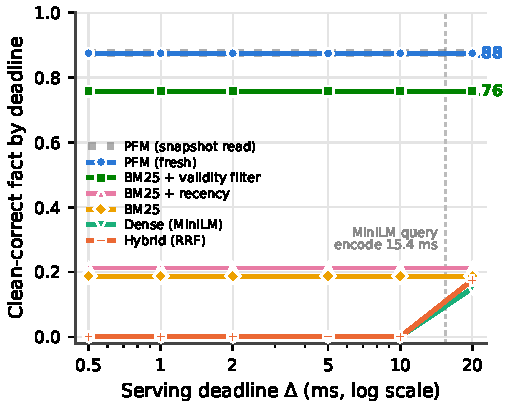
\includegraphics[width=\columnwidth]{figures/deadline_curve.pdf}
\caption{Fraction of requests that obtain a clean correct fact within a serving deadline $\Delta$, on the update benchmark. Validity-aware lexical serving is deadline-insensitive across the interactive range; the snapshot path is deadline-independent by construction and its curve coincides with PFM (fresh) at these deadlines; the local dense retriever cannot meet any deadline below its query-encoding cost (p50 15.4~ms) regardless of ranking quality.}
\label{fig:deadline}
\end{figure}

Table~\ref{tab:baselines} and Figure~\ref{fig:deadline} support three conclusions. \emph{Temporal correctness is set by the write path, not the ranker}: both validity-aware arms exceed .75 clean while every validity-agnostic arm stays below .27, and giving plain BM25 the same validity bits recovers most of the gap---PFM's field weighting adds the rest, lifting current-value recall from .892 to 1.000 on the associative and participant-dependent queries. \emph{Representational power does not substitute for temporal state}: the dense retriever has the best current-value recall (.975) yet the worst stale exposure (.779), because embedding similarity ranks every version of a revised fact near the query. \emph{The deadline separates methods that accuracy alone cannot}: MiniLM query encoding costs 15.4~ms, so dense and hybrid deliver zero clean facts within a 10~ms deadline (under 18 percent within 20~ms), whereas PFM's fresh path serves its full clean rate from 0.5~ms and the snapshot path is deadline-independent by construction. Deadline-constrained clean retrieval thus requires both validity-aware construction and a serving path whose cost is below the deadline.

\subsection{Completion-Level Evidence with a Frozen Local Model}

Fact availability establishes that information reached the prompt, not that it changed the completion. We therefore replay a stratified sample of 120 benchmark queries (weighted toward revised and ambiguous chains) through a frozen local model, qwen2:7b served by ollama on the same machine, with temperature 0 and identical decoding across arms. Each request assembles the same prompt the assistant would use---typing context, participant, and the arm's retrieved memory block---and the generated completion is judged by normalized containment: \emph{correct} when it contains the current value, \emph{stale} when it instead contains a superseded value, \emph{wrong-person} when it contains a same-first-name competitor's value, and \emph{other} otherwise. We also record time to first streamed token (TTFT).

\begin{table}[t]
\centering
\small
\begin{tabular}{@{}lrrrrr@{}}
\toprule
Memory & Correct & Stale & Wrong & Other & TTFT \\
 & & & pers. & & p50 (ms) \\
\midrule
None        & .000 & .000 & .000 & 1.000 & 296 \\
PFM         & \textbf{.925} & .000 & .000 & .075 & 1194 \\
BM25 (plain) & .517 & .358 & .008 & .117 & 1036 \\
\bottomrule
\end{tabular}
\caption{Frozen-LLM replay (qwen2:7b, 120 queries, temperature 0). Correct CI for PFM: (.864, .960); stale CI for plain BM25: (.278, .447). The upper bound on PFM stale and wrong-person generations is 3.1 percent.}
\label{tab:llm}
\end{table}

Table~\ref{tab:llm} shows that prompt-side differences propagate to generations. Without memory, the model produces the labeled value on none of 120 requests; every completion is a guess. With PFM's block, 92.5 percent of completions contain the current value and none contain a stale or wrong-person value. With plain BM25's block, 51.7 percent are correct and 35.8 percent reproduce a superseded value: stale facts in the prompt become stale text in the output at a rate close to the block's stale-exposure rate. Notably, wrong-person exposure does not translate into wrong-person generation: although a same-first-name competitor's fact enters the prompt on 12.5 percent of benchmark queries, the model selects the correctly attributed fact in every sampled case, so prompt-level exposure and completion-level error are related but not identical. The injected block also carries a prefill cost---time to first token rises from 296~ms to about 1.2~s with an 800-character block on this 7B CPU configuration; per-outcome intervals and the full judging breakdown are in the supplement. These results are specific to one model, one decoding configuration, and a containment judge; they establish that retrieved facts change completions, not that users accept them.

\paragraph{Latency and scaling.} On the deployed replay store, measured on a single Apple Silicon thread, median retrieval latency is 0.011~ms at 270 facts (p95 0.024~ms) and 1.81~ms at 20{,}000 facts (p95 2.03~ms). Across store sizes from 100 to 100{,}000 synthetic facts on a fixed hardware profile, per-fact update cost stays near 0.1~ms while fresh-retrieval latency grows with posting-list density, reaching 12.5~ms at 20{,}000 facts and 81~ms at 100{,}000 facts on a deliberately dense distribution. Under snapshot serving the completion path remains a single bounded read regardless of store size, at the cost of snapshot freshness. The full scaling grid, hardware, thread situation, and timing boundaries are reported in the supplement, together with component ablations of the replay retriever (participant field, entity graph, and recency decay) and the detailed update-benchmark breakdowns referenced above.

\section{Limitations}

The controlled evidence in this paper stops short of live product impact. The update benchmark, the baseline comparison, and the frozen-model replay are built from template-generated corpora whose value tokens are globally unique by construction; real personal text is noisier, and paraphrase in the benchmark spans a fixed template family rather than unconstrained rewording. The completion-level study uses one frozen model, one decoding configuration, and a normalized-containment judge; it establishes that retrieved facts change generated text, not that users accept the resulting completions or benefit over long-running personal histories.

Temporal versioning depends on the construction path recognizing that two observations refer to the same mutable slot. The key-emitting extractor evaluated here achieves this on the benchmark's six slot types, and correcting its slot detection required value-type constraints precisely because noun families overlap across slots---evidence that key assignment is the fragile step. Proposition~\ref{prop:unique_active_value} characterizes consistency after revisions receive a common key; it does not guarantee revision detection on unconstrained natural text, and the extractor shipped in the deployed assistant has not yet adopted the keyed rules, so deployed behavior currently matches the keyless arm of Table~\ref{tab:temporal}.

Several components remain only partially identified, and the systems numbers carry stated scope. Removing the entity graph or recency decay does not change availability on the 25 replay scenarios, so their necessity is not established there. Under identity ambiguity with $k{=}6$ slots, a same-first-name competitor's fact still enters the prompt on 12.5\% of benchmark queries even though the frozen model selected the correctly attributed fact in every sampled case; exposure-level ambiguity is unresolved at the retrieval layer. A scaling grid (supplement) shows that fresh-retrieval latency is governed by term-frequency structure rather than fact count alone, reaching 81~ms at 100{,}000 dense synthetic facts in the reference implementation; snapshot serving hides this from the completion path but not from snapshot freshness, and index-side mitigation at that scale is future work. All latency measurements are from one Apple Silicon machine with a single retrieval thread.

\section{Conclusion}

We formulated deadline-constrained personal fact retrieval, in which a personal memory layer must return relevant information that is correctly attributed, still valid, and available before generation begins. PFM addresses this setting with participant-aware atomic facts, keyed temporal supersession applied before duplicate admission, asynchronous memory construction, and an in-memory serving path that does not invoke an embedding model or language model. The evaluation supports three conclusions. Temporal correctness is a property of the write path: keyed supersession takes stale exposure from 66.2\% to zero on a 240-query update benchmark, and even plain BM25 recovers most of the clean-retrieval gap when given the same validity information, while no validity-agnostic retriever exceeds a .27 clean rate. The serving deadline separates methods that accuracy alone cannot: a local dense retriever with the best current-value recall of any baseline delivers zero clean facts within a 10~ms deadline because of its query-encoding cost, while PFM serves its full clean rate from 0.5~ms and its snapshot path is deadline-independent by construction. Finally, prompt-side correctness propagates to generations: with a frozen 7B model, correct completions rise from 0\% to 92.5\% with PFM and stale prompts become stale text for validity-agnostic retrieval. Personal memory should therefore be evaluated for misattribution, staleness, and lateness separately, at both the prompt and the completion level, rather than through retrieval accuracy alone.

% --- Bibliography --------------------------------------------------------
\bibliographystyle{aaai27}   % from the Author Kit
\bibliography{aaai2027}      % aaai2027.bib in this folder

\end{document}
